% !TeX program = xelatex
\documentclass[a4paper,10pt]{article}

% ============================================================================
% សន្លឹកកិច្ចការសិស្សបំពេញចន្លោះ ស-ខ្មៅ និងប្លង់ក្ដារខៀន/ចម្លើយគ្រូ (គ្មាន LCD / គ្មានកន្ត្រៃ)
% មេរៀនទី៤ (៣)៖ ម៉ាសធៀបនឹងមាឌ — ត្រូវគ្នា ១០០% នឹង LS_Plan_MEAS43.tex
% ============================================================================
\usepackage[a4paper, left=1.0cm, right=1.0cm, top=0.75cm, bottom=1.00cm, footskip=0.52cm]{geometry}
\usepackage{amsmath}
\usepackage{unicode-math}
\usepackage{fontspec}
\usepackage{array, colortbl}
\usepackage[table]{xcolor}
\usepackage{enumitem}
\usepackage{pifont}
\usepackage{fancyhdr}
\usepackage{lastpage}
\usepackage{tikz}
\usepackage[most]{tcolorbox}
\usetikzlibrary{calc, arrows.meta, decorations.pathreplacing, positioning, babel}

\makeatletter
\let\@expl@@@mark@update@singlecol@structures@@\relax
\makeatother

\providecommand{\NGSFindFonts}{%
  \IfFileExists{C:/Windows/Fonts/cambria.ttc}{%
    \def\NGSSysPath{C:/Windows/Fonts/}%
    \def\NGSUserPath{C:/Users/KIT/AppData/Local/Microsoft/Windows/Fonts/}%
  }{%
    \IfFileExists{./fonts/KhmerOSsiemreap.ttf}{\def\NGSSysPath{./fonts/}\def\NGSUserPath{./fonts/}}{%
    \IfFileExists{../fonts/KhmerOSsiemreap.ttf}{\def\NGSSysPath{../fonts/}\def\NGSUserPath{../fonts/}}{%
    \IfFileExists{../../fonts/KhmerOSsiemreap.ttf}{\def\NGSSysPath{../../fonts/}\def\NGSUserPath{../../fonts/}}{%
    \IfFileExists{../../../fonts/KhmerOSsiemreap.ttf}{\def\NGSSysPath{../../../fonts/}\def\NGSUserPath{../../../fonts/}}{%
    \IfFileExists{../../../../fonts/KhmerOSsiemreap.ttf}{\def\NGSSysPath{../../../../fonts/}\def\NGSUserPath{../../../../fonts/}}{%
    \IfFileExists{../../../../../fonts/KhmerOSsiemreap.ttf}{\def\NGSSysPath{../../../../../fonts/}\def\NGSUserPath{../../../../../fonts/}}{%
    \IfFileExists{../../../../../../fonts/KhmerOSsiemreap.ttf}{\def\NGSSysPath{../../../../../../fonts/}\def\NGSUserPath{../../../../../../fonts/}}{%
      \def\NGSSysPath{../../../../../../../fonts/}\def\NGSUserPath{../../../../../../../fonts/}%
    }}}}}}}%
  }%
}
\NGSFindFonts

\setmathfont[Path={\NGSSysPath}, FontIndex=1, Scale=1.02]{cambria.ttc}
\defaultfontfeatures{Ligatures=TeX}

\setmainfont[
  Path={\NGSUserPath}, Extension=.ttf, Script=Khmer,
  BoldFont={KhmerOSsiemreap}, BoldFeatures={FakeBold=1.8},
  ItalicFont={KhmerOSsiemreap}, ItalicFeatures={FakeSlant=0.25},
  BoldItalicFont={KhmerOSsiemreap}, BoldItalicFeatures={FakeBold=1.8, FakeSlant=0.25}
]{KhmerOSsiemreap}

\newfontfamily\muol[Path={\NGSUserPath}, Extension=.ttf, Script=Khmer]{KhmerOSmuollight}
\newfontfamily\TimesEn[Path={\NGSSysPath}, Extension=.ttf, BoldFont={timesbd}, ItalicFont={timesi}, BoldItalicFont={timesbi}]{times}
\newfontfamily\CalibriFont[Path={\NGSSysPath}, Extension=.ttf]{calibri}

\XeTeXlinebreaklocale "km"
\XeTeXlinebreakskip = 0pt plus 1pt minus 0.1pt

\definecolor{panelgray}{gray}{0.94}
\definecolor{headgray}{gray}{0.85}

\pagestyle{fancy}
\fancyhf{}
\renewcommand{\headrulewidth}{0pt}
\fancyfoot[L]{\fontsize{7.4pt}{9.5pt}\selectfont អនុវិទ្យាល័យព្រះក្រសាំង \en{|} គ្រូ៖ ហុក ប៊ុនថែន \en{|} មេរៀនទី៤ (៣) ម៉ាសធៀបនឹងមាឌ \en{|} ថ្ងៃពុធ ទី២ ខែធ្នូ ឆ្នាំ២០២៦}
\fancyfoot[R]{\fontsize{7.8pt}{10pt}\selectfont ទំព័រ \en{\thepage\ / \pageref{LastPage}}}

\setlength{\parindent}{0pt}
\setlength{\parskip}{0pt}
\setlength{\tabcolsep}{4pt}

\newcommand{\en}[1]{{\TimesEn #1}}
\newcommand{\enbf}[1]{{\TimesEn\bfseries #1}}
\newcommand{\unit}[1]{\,\text{\en{#1}}}
\newcommand{\riel}{\,\text{៛}}
\newcommand{\cnum}[1]{\mbox{\fontsize{10pt}{12pt}\selectfont\ding{\numexpr181+#1\relax}}}
\newcommand{\chkbox}{\tikz[baseline=-0.15ex]\draw[black, line width=0.85pt, fill=white] (0,0) rectangle (0.24cm,0.24cm);}
\newcommand{\ansbox}[1][1.75cm]{\,\tikz[baseline=-0.65ex]\draw[black, line width=0.65pt, fill=white] (0,0) rectangle (#1, 0.42cm);\,}
\newcommand{\dotline}[1][2.2cm]{\makebox[#1]{\dotfill}}

\newcommand{\pagebanner}[2]{%
  \begin{tcolorbox}[
    enhanced, sharp corners, colback=headgray, colframe=black,
    boxrule=1.05pt, boxsep=1pt, top=2.5pt, bottom=2.5pt, left=6pt, right=6pt,
    after skip=3.5pt
  ]
    {\muol\fontsize{9.0pt}{13.2pt}\selectfont #1}\hfill{\fontsize{8.0pt}{11.2pt}\selectfont\textbf{#2}}
  \end{tcolorbox}%
}

\newcommand{\secstrip}[2]{%
  \vspace{3pt}%
  \begin{tcolorbox}[
    enhanced, sharp corners, colback=panelgray, colframe=black,
    boxrule=0.8pt, boxsep=0.8pt, top=2pt, bottom=2pt, left=5pt, right=5pt,
    after skip=3pt
  ]
    {\muol\fontsize{8.5pt}{12.2pt}\selectfont #1}\hfill{\fontsize{7.8pt}{10.8pt}\selectfont\textit{#2}}
  \end{tcolorbox}%
}

\newcolumntype{L}[1]{>{\raggedright\arraybackslash}p{#1}}
\newcolumntype{C}[1]{>{\centering\arraybackslash}p{#1}}

\begin{document}
\fontsize{9.5pt}{14.5pt}\selectfont

% ============================================================================
% ទំព័រទី ១៖ សន្លឹកកិច្ចការសិស្ស (ផ្នែកមុខ៖ E1 -> E2 -> E3)
% ============================================================================
\pagebanner{សន្លឹកកិច្ចការសិស្ស \enbf{(}៤\enbf{.}៣ ម៉ាសធៀបនឹងមាឌ\enbf{)} \enbf{--} ផ្នែកមុខ}{ថ្នាក់ទី៨ \en{|} សៀវភៅគោល ទំ.៤៦--៤៧}

\begin{tcolorbox}[
  enhanced, sharp corners, colback=white, colframe=black,
  boxrule=0.8pt, boxsep=1.5pt, top=3.5pt, bottom=3.5pt, left=5pt, right=5pt,
  after skip=4pt
]
  \fontsize{9.0pt}{13.0pt}\selectfont
  \textbf{ឈ្មោះសិស្ស៖} \dotline[4.3cm] \quad
  \textbf{សមាជិកក្រុម៖} \dotline[4.3cm] \quad
  \textbf{ថ្នាក់ទី៖} ៨\dotline[0.9cm] \quad
  \textbf{ក្រុមទី៖} \dotline[1.0cm]
\end{tcolorbox}

% --- E1 Engage ---
\secstrip{ផ្នែកទី ១ \enbf{(E1 - Engage)} ៖ បេសកកម្មជាងសំណង់ស្ទង់ទម្ងន់ដែកសរសៃ}{រយៈពេល ៣ នាទី (គូស \ding{51} ក្នុង \chkbox)}

\begin{tcolorbox}[
  enhanced, sharp corners, colback=white, colframe=black,
  boxrule=0.8pt, boxsep=2pt, top=3.5pt, bottom=3.5pt, left=6pt, right=6pt
]
  នៅការដ្ឋានសំណង់ ដែក $6$ លី ($d = 6\unit{mm}$) មួយដើមប្រវែង $12\unit{m}$ មានម៉ាសប្រហែល $2.67\unit{kg}$ ។ ចុះដែក $12$ លី ($d = 12\unit{mm}$, $l = 12\unit{m}$)៖\\[2pt]
  $\bullet$ \textbf{តើជាងរូបណាប៉ាន់ស្មានទម្ងន់ដែក $12$ លី បានត្រឹមត្រូវ?} \quad
  \chkbox\ \textbf{ជាង ក៖} ធ្ងន់ $2$ ដង ($\approx 5.34\unit{kg}$) \qquad
  \chkbox\ \textbf{ជាង ខ៖} ធ្ងន់ $4$ ដង ($\approx 10.7\unit{kg}$)\\[2pt]
  $\bullet$ \textbf{ហេតុផលខ្លី៖} ក្នុងរូបមន្តមាឌស៊ីឡាំង $V = \frac{\pi d^2}{4}\times l$ អង្កត់ផ្ចិត $d$ មានស្វ័យគុណស្មើ \dotline[2.4cm] ។
\end{tcolorbox}

\vfill

% --- E2 Explore ---
\secstrip{ផ្នែកទី ២ \enbf{(E2 - Explore)} ៖ ម៉ាសមាឌលោហធាតុ និងលំហាត់គំរូទី ១ (ទំ.៤៦--៤៧)}{រយៈពេល ១១ នាទី}

\textbf{សកម្មភាព ១ (\en{E2-A} — ៦ នាទី)៖ បំប្លែងម៉ាសមាឌ $\mu$ និងគណនាម៉ាសដែក $10$ លី និង $12$ លី ($l = 12\unit{m}, \pi = 3.14$)}

\begin{tcolorbox}[
  enhanced, sharp corners, colback=white, colframe=black,
  boxrule=0.8pt, boxsep=2pt, top=3.5pt, bottom=3.5pt, left=6pt, right=6pt
]
  $\bullet$ \textbf{បំប្លែងម៉ាសមាឌដែក (ទំ.៤៦--៤៧)៖} $\mu = 7.874\unit{g/cm}^3 = \dfrac{7.874\times 10^{-3}\unit{kg}}{(10^{-2}\unit{m})^3} = \dfrac{7.874\times 10^{-3}}{10^{-6}}\unit{kg/m}^3 =$ \ansbox[2.2cm] $\unit{kg/m}^3$\\[3pt]
  $\bullet$ \textbf{១) ដែក $10$ លីមួយដើម ($d = 10\unit{mm} = 10\times 10^{-3}\unit{m} \implies d^2 = 100\times 10^{-6}\unit{m}^2$)៖}\\[2pt]
  \hspace*{0.3cm}$m_{10} = \dfrac{\pi d^2}{4}\times l\times \mu = 3.14\times \dfrac{100\times 10^{-6}}{4}\times 12\times 7\,874 =$ \dotline[2.2cm] $\unit{kg} \approx$ \ansbox[1.8cm] $\unit{kg}$\\[3pt]
  $\bullet$ \textbf{២) ដែក $12$ លីមួយដើម ($d = 12\unit{mm} = 12\times 10^{-3}\unit{m} \implies d^2 =$ \dotline[2.0cm] $\unit{m}^2$)៖}\\[2pt]
  \hspace*{0.3cm}$m_{12} = 3.14\times \dfrac{\dotline[1.9cm]}{4}\times 12\times 7\,874 =$ \dotline[2.2cm] $\unit{kg} \approx$ \ansbox[1.8cm] $\unit{kg}$
\end{tcolorbox}

\vspace{3pt}
\textbf{សកម្មភាព ២ (\en{E2-B} — ៥ នាទី)៖ ពិនិត្យអន្ទាក់បំប្លែងខ្នាតសមាស $\unit{g/cm}^3$ និងអន្ទាក់អង្កត់ផ្ចិត $d^2$}

\begin{tcolorbox}[
  enhanced, sharp corners, colback=white, colframe=black,
  boxrule=0.8pt, boxsep=2pt, top=3.5pt, bottom=3.5pt, left=6pt, right=6pt
]
  $\bullet$ \textbf{អន្ទាក់ខ្នាតសមាស៖} $1\unit{g/cm}^3 =$ \dotline[1.6cm] $\unit{kg/m}^3$ ដូចនេះម៉ាសមាឌស្ពាន់ $8.94\unit{g/cm}^3 =$ \dotline[1.8cm] $\unit{kg/m}^3$ ។\\[2.5pt]
  $\bullet$ \textbf{អន្ទាក់អង្កត់ផ្ចិត៖} ធៀបនឹងដែក $6$ លី ($2.67\unit{kg}$) ដែក $12$ លី ($10.68\unit{kg}$) ធ្ងន់ជាង $\left(\dfrac{12}{6}\right)^2 =$ \dotline[1.0cm] ដង!
\end{tcolorbox}

\vfill

% --- E3 Explain ---
\secstrip{ផ្នែកទី ៣ \enbf{(E3 - Explain)} ៖ រូបមន្តម៉ាសមាឌ និងធនាគារហេតុផល \enbf{B\&W}}{រយៈពេល ៦ នាទី}

\begin{tcolorbox}[
  enhanced, sharp corners, colback=white, colframe=black,
  boxrule=0.85pt, boxsep=2pt, top=3.5pt, bottom=3.5pt, left=6pt, right=6pt
]
  ១) \textbf{បំប្លែងខ្នាត៖} $1\unit{g/cm}^3 =$ \dotline[1.4cm] $\unit{kg/m}^3$ \qquad
  ២) \textbf{ម៉ាសវត្ថុ៖} $m = V \times \dotline[0.9cm]$ \qquad
  ៣) \textbf{ម៉ាសស៊ីឡាំង៖} $m = \dfrac{\pi d^2}{4}\times l\times \dotline[0.9cm]$\\[4pt]
  \tikz\draw[black, dashed, line width=0.5pt] (0,0) -- (18.4cm,0);\\[3pt]
  \fontsize{8.8pt}{12.8pt}\selectfont
  \textbf{ធនាគារហេតុផល (\en{Warrant Bank})៖} \quad
  \cnum{1} \textbf{ខ្នាត $\mu$៖} $1\unit{g/cm}^3 = 1\,000\unit{kg/m}^3$ (ដែក $7\,874$, ស្ពាន់ $8\,940$, ប្រាក់ $10\,490$, មាស $19\,300\unit{kg/m}^3$)\\
  \cnum{2} \textbf{ដែក $k$ លី៖} $d = k\times 10^{-3}\unit{m} \implies d^2 = k^2\times 10^{-6}\unit{m}^2$ \quad
  \cnum{3} \textbf{ម៉ាសសរសៃ៖} $m = \frac{\pi d^2}{4}\times l\times \mu$ \quad
  \cnum{4} \textbf{ផលធៀប៖} $\frac{m_2}{m_1} = \left(\frac{d_2}{d_1}\right)^2$
\end{tcolorbox}

% ============================================================================
% ទំព័រទី ២៖ សន្លឹកកិច្ចការសិស្ស (ផ្នែកខាងខ្នង៖ E4 -> E5 -> កិច្ចការផ្ទះ)
% ============================================================================
\clearpage
\pagebanner{សន្លឹកកិច្ចការសិស្ស \enbf{(}៤\enbf{.}៣ ម៉ាសធៀបនឹងមាឌ\enbf{)} \enbf{--} ផ្នែកខាងខ្នង}{ថ្នាក់ទី៨ \en{|} សៀវភៅគោល ទំ.៤៧--៤៨, ៥០}

% --- E4 Elaborate ---
\secstrip{ផ្នែកទី ៤ \enbf{(E4 - Elaborate)} ៖ ដែក $14$ លី និងលំហាត់គំរូទី ២ — មាឌដែក $12$ លី (ទំ.៤៧--៤៨)}{រយៈពេល ១០ នាទី}

\begin{tcolorbox}[
  enhanced, sharp corners, colback=white, colframe=black,
  boxrule=0.8pt, boxsep=2pt, top=3.5pt, bottom=3.5pt, left=6pt, right=6pt
]
  \textbf{១) គណនាម៉ាសដែក $14$ លី មួយដើម ($l = 12\unit{m}, \mu = 7\,874\unit{kg/m}^3, \pi = 3.14$ — ទំ.៤៧)៖}\\[2.5pt]
  $\bullet$ អង្កត់ផ្ចិត (\cnum{2})៖ $d = 14\unit{mm} = 14\times 10^{-3}\unit{m} \implies d^2 =$ \dotline[2.3cm] $\unit{m}^2$\\[3pt]
  $\bullet$ ម៉ាស (\cnum{3})៖ $m_{14} = 3.14\times \dfrac{d^2}{4}\times 12\times 7\,874 =$ \dotline[2.2cm] $\unit{kg} \approx$ \ansbox[1.8cm] $\unit{kg}$\\[3pt]
  \textbf{២) លំហាត់គំរូទី ២ (ទំ.៤៧--៤៨)៖} គណនាមាឌដែកគិតជា $\unit{m}^3$ ដោយដឹងថាដែក $12$ លីមួយដើមមានប្រវែង $l = 12\unit{m}$ ($\pi = 3.14$)៖\\[2.5pt]
  $\bullet$ $V = S\times l = \dfrac{\pi d^2}{4}\times l = \dfrac{3.14\times 144\times 10^{-6}}{4}\times 12 \approx$ \ansbox[3.0cm] $\unit{m}^3$\\[2pt]
  \fontsize{8.7pt}{12.5pt}\selectfont
  \textbf{ឆ្លុះបញ្ចាំង (\en{EIA Looking-Back})៖} ផ្ទៀង $V\times \mu = 1\,356.48\times 10^{-6}\times 7\,874 \approx$ \dotline[1.6cm] $\unit{kg}$ (ត្រូវគ្នានឹង $m_{12}$!) ។
\end{tcolorbox}

\vfill

% --- E5 Evaluate ---
\secstrip{ផ្នែកទី ៥ \enbf{(E5 - Evaluate)} ៖ លំហាត់ប្រតិបត្តិពូសុខ (ទំ.៤៨) សំណួរវិនិច្ឆ័យ \enbf{A--D} និងសំបុត្រចេញ}{រយៈពេល ១០ នាទី}

\begin{tcolorbox}[
  enhanced, sharp corners, colback=white, colframe=black,
  boxrule=0.8pt, boxsep=2pt, top=3.5pt, bottom=3.5pt, left=6pt, right=6pt
]
  \textbf{១) ប្រតិបត្តិ (ទំ.៤៨)៖} ពូសុខទិញដែក $6$ លី ចំនួន $200$ ដើម និងដែក $10$ លី ចំនួន $20$ ដើម ($l = 12\unit{m}, \mu = 7.874\unit{g/cm}^3$) ។ បើដែក $1\unit{kg}$ ថ្លៃ $2\,800\riel$ គណនាប្រាក់ដែលពូសុខទិញដែកទាំងពីរមុខនោះ៖\\[3pt]
  $\bullet$ ដែក $6$ លី៖ ១ ដើម $m_6 \approx$ \dotline[1.8cm] $\unit{kg} \implies 200$ ដើម $\approx$ \dotline[2.0cm] $\unit{kg}$\\[3pt]
  $\bullet$ ដែក $10$ លី៖ ១ ដើម $m_{10} \approx$ \dotline[1.8cm] $\unit{kg} \implies 20$ ដើម $\approx$ \dotline[2.0cm] $\unit{kg}$\\[3pt]
  $\bullet$ ម៉ាសសរុប $m \approx$ \dotline[2.0cm] $\unit{kg} \implies$ ប្រាក់ចំណាយ $= m\times 2\,800 \approx$ \ansbox[2.8cm] $\riel$\\[3pt]
  \textbf{២) បិទបេសកកម្ម \en{E1}៖} ជាង \dotline[0.9cm] ត្រឹមត្រូវ ព្រោះដែក $12$ លី ធ្ងន់ប្រហែល \dotline[1.5cm] $\unit{kg}$ (ធ្ងន់ជាងដែក $6$ លី ចំនួន $4$ ដង) ។
\end{tcolorbox}

\vspace{3.5pt}

\begin{tcolorbox}[
  enhanced, sharp corners, colback=white, colframe=black,
  boxrule=0.8pt, boxsep=2pt, top=3.5pt, bottom=3.5pt, left=6pt, right=6pt
]
  \textbf{៣) សំណួរវិនិច្ឆ័យ \en{A--D} (ដុំមាសសុទ្ធមានមាឌ $V = 100\unit{cm}^3 = 10^{-4}\unit{m}^3$, $\mu_{\text{មាស}} = 19.3\unit{g/cm}^3$ តើមានម៉ាសប៉ុន្មាន $\unit{kg}$? — លើកម្រាមដៃ ១--៤)៖}\\[2.5pt]
  \textbf{\en{A.}} $1\,930\unit{kg}$ \qquad
  \textbf{\en{B.}} $1.93\unit{kg}$ \qquad
  \textbf{\en{C.}} $0.00193\unit{kg}$ \qquad
  \textbf{\en{D.}} $19.3\unit{kg}$\\[3.5pt]
  \tikz\draw[black, dashed, line width=0.5pt] (0,0) -- (18.4cm,0);\\[3pt]
  \textbf{៤) សំបុត្រចេញ ៦០ វិនាទី៖} ម៉ាសមាឌស្ពាន់ $\mu = 8.94\unit{g/cm}^3 =$ \dotline[1.8cm] $\unit{kg/m}^3$;
  បើដុំស្ពាន់មានមាឌ $V = 2\times 10^{-3}\unit{m}^3 \implies m =$ \dotline[1.8cm] $\unit{kg}$ ។
\end{tcolorbox}

\vfill

% --- Homework ---
\begin{tcolorbox}[
  enhanced, sharp corners, colback=panelgray, colframe=black,
  boxrule=0.95pt, boxsep=2pt, top=3.5pt, bottom=3.5pt, left=6pt, right=6pt
]
  {\muol\fontsize{9.0pt}{13.0pt}\selectfont កិច្ចការផ្ទះ \enbf{(}សៀវភៅគោល ទំ.៥០ លេខ ៤ និង លេខ ៦\enbf{)}}\\[2.5pt]
  \fontsize{8.8pt}{13.0pt}\selectfont
  $\bullet$ \textbf{\#4 (ទំ.៥០)៖} គេដឹងថាដែក $10$ លីមួយដើមមានម៉ាស $7.4\unit{kg}$ ។ ចូររកម៉ាសនៃដែក $16$ លីវិញ ។\\
  $\bullet$ \textbf{\#6 (ទំ.៥០)៖} ខ្សែភ្លើងមួយដុំមានប្រវែង $100\unit{m}$ មានមុខកាត់ (អង្កត់ផ្ចិត) $2\frac{1}{2}\unit{mm}$ ($= 2.5\unit{mm}$) ។ គណនាម៉ាសនៃខ្សែភ្លើងនេះដោយដឹងថាម៉ាសមាឌនៃស្ពាន់ខ្សែភ្លើង $\mu = 8.94\unit{g/cm}^3$ ($\pi = 3.14$, មិនគិតម៉ាសជ័រស្រោបទេ) ។ \textbf{អានមុន៖} ៤. ល្បឿនមធ្យម (ទំ.៤៨--៤៩) ។
\end{tcolorbox}

% ============================================================================
% ទំព័រទី ៣៖ ទំព័រគ្រូបង្រៀន (គំរូប្លង់ក្ដារខៀន ៣ ផ្នែក + ចម្លើយផ្ទៀងផ្ទាត់រហ័ស)
% ============================================================================
\clearpage
\pagebanner{ទំព័រគ្រូបង្រៀន ៖ ប្លង់ក្ដារខៀន \enbf{(}គ្មាន \enbf{LCD)} និងចម្លើយផ្ទៀងផ្ទាត់រហ័ស}{៤.៣ ម៉ាសធៀបនឹងមាឌ (\en{MEAS43})}

\secstrip{១. គំរូប្លង់បែងចែកក្ដារខៀន ៣ ផ្នែក សម្រាប់ថ្នាក់រៀនគ្មាន \enbf{LCD}}{សម្រាប់គ្រូប្រើដីស/ហ្វឺត}

\begin{center}
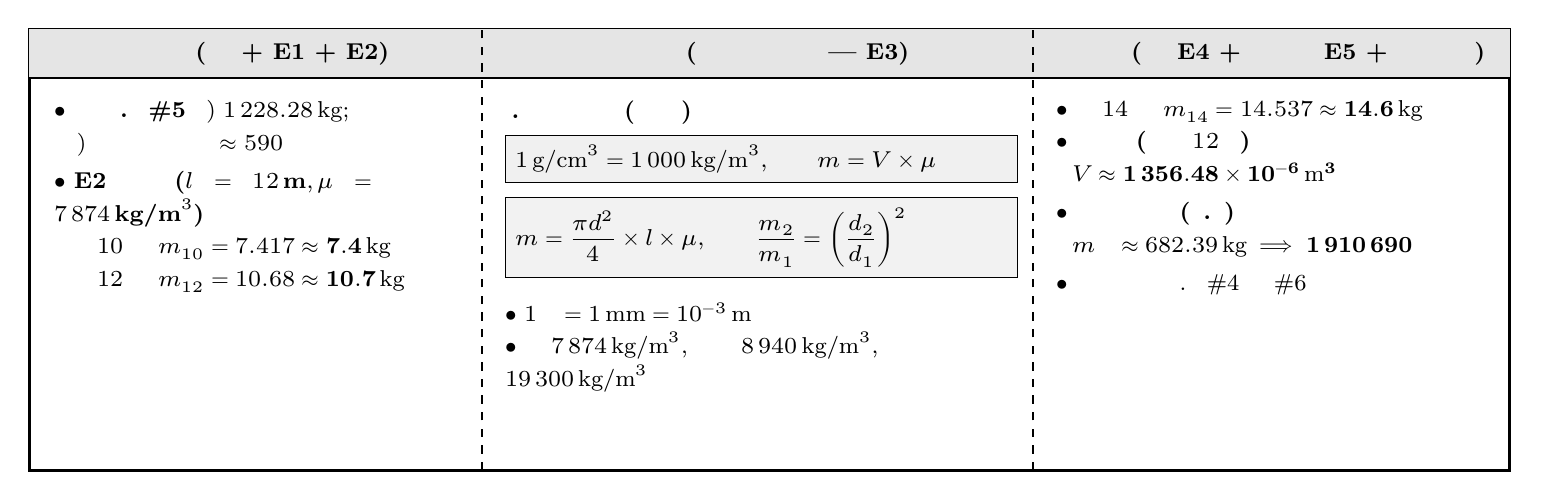
\begin{tikzpicture}[x=1cm, y=1cm, every node/.style={font=\fontsize{8.3pt}{11.8pt}\selectfont, text=black}]
  \draw[black, line width=1.1pt] (0,0) rectangle (18.8,5.60);
  \fill[gray!20] (0,4.98) rectangle (18.8,5.60);
  \draw[black, line width=0.7pt] (0,4.98) -- (18.8,4.98);
  \draw[black, dashed, line width=0.7pt] (5.75,0) -- (5.75,5.60);
  \draw[black, dashed, line width=0.7pt] (12.75,0) -- (12.75,5.60);

  \node at (2.875,5.29) {\textbf{ផ្នែកឆ្វេង (កំណែ + \en{E1} + \en{E2})}};
  \node at (9.25,5.29) {\textbf{ផ្នែកកណ្ដាល (ខ្លឹមសារគោលរក្សាទុក — \en{E3})}};
  \node at (15.775,5.29) {\textbf{ផ្នែកស្ដាំ (គំរូ \en{E4} + ប្រតិបត្តិ \en{E5} + កិច្ចការផ្ទះ)}};

  % Left
  \node[anchor=north west, text width=5.35cm] at (0.20,4.82) {%
    $\bullet$ \textbf{កំណែ ទំ.៥០ \#5៖} ក) $1\,228.28\unit{kg}$;\\
    \hspace*{0.2cm}ខ) ថ្លៃក្រដាស ១ ក្បាល $\approx 590\riel$\\[2pt]
    $\bullet$ \textbf{\en{E2} គំរូទី ១ ($l=12\unit{m}, \mu=7\,874\unit{kg/m}^3$)៖}\\
    \hspace*{0.2cm}ដែក $10$ លី៖ $m_{10} = 7.417 \approx \mathbf{7.4\unit{kg}}$\\
    \hspace*{0.2cm}ដែក $12$ លី៖ $m_{12} = 10.68 \approx \mathbf{10.7\unit{kg}}$
  };

  % Center
  \node[anchor=north west, text width=6.65cm] at (5.92,4.82) {%
    {\muol\fontsize{8.5pt}{12pt}\selectfont ៣\enbf{.} ម៉ាសធៀបនឹងមាឌ \enbf{(}ម៉ាសមាឌ\enbf{)}}\\[3pt]
    \tikz\node[draw=black, fill=gray!12, inner sep=3.5pt, text width=6.25cm]{%
      $1\unit{g/cm}^3 = 1\,000\unit{kg/m}^3, \qquad m = V\times \mu$
    };\\[4pt]
    \tikz\node[draw=black, fill=gray!10, inner sep=3.5pt, text width=6.25cm]{%
      $m = \dfrac{\pi d^2}{4}\times l\times \mu, \qquad \dfrac{m_2}{m_1} = \left(\dfrac{d_2}{d_1}\right)^2$
    };\\[4pt]
    $\bullet$ $1\text{ លី} = 1\unit{mm} = 10^{-3}\unit{m}$\\
    $\bullet$ ដែក $7\,874\unit{kg/m}^3$, ស្ពាន់ $8\,940\unit{kg/m}^3$, មាស $19\,300\unit{kg/m}^3$
  };

  % Right
  \node[anchor=north west, text width=5.8cm] at (12.92,4.82) {%
    $\bullet$ \textbf{ដែក $14$ លី៖} $m_{14} = 14.537 \approx \mathbf{14.6\unit{kg}}$\\
    $\bullet$ \textbf{គំរូទី ២ (មាឌដែក $12$ លី)៖}\\
    \hspace*{0.2cm}$V \approx \mathbf{1\,356.48\times 10^{-6}\unit{m}^3}$\\[2pt]
    $\bullet$ \textbf{ប្រតិបត្តិពូសុខ (ទំ.៤៨)៖}\\
    \hspace*{0.2cm}$m_{\text{សរុប}} \approx 682.39\unit{kg} \implies \mathbf{1\,910\,690\riel}$\\[2pt]
    $\bullet$ \textbf{កិច្ចការផ្ទះ៖} ទំ.៥០ \#4 និង \#6
  };
\end{tikzpicture}
\end{center}

\vspace{4pt}
\secstrip{២. ចម្លើយផ្ទៀងផ្ទាត់រហ័សសម្រាប់សន្លឹកកិច្ចការសិស្ស \enbf{(}ទំព័រ ១ និង ទំព័រ ២\enbf{)}}{\en{Answer Key}}

\begin{tcolorbox}[
  enhanced, sharp corners, colback=white, colframe=black,
  boxrule=0.8pt, boxsep=2pt, top=4pt, bottom=4pt, left=6pt, right=6pt
]
  \fontsize{9.0pt}{13.6pt}\selectfont
  $\bullet$ \textbf{ផ្នែក \en{E1}៖} \textbf{ជាង ខ} ត្រឹមត្រូវ ព្រោះក្នុងរូបមន្តមាឌស៊ីឡាំង $d$ មានស្វ័យគុណ $2$ ធ្វើឱ្យម៉ាសកើន $2^2 = 4$ ដង ($\approx 10.7\unit{kg}$) ។\\[2pt]
  $\bullet$ \textbf{ផ្នែក \en{E2}៖} \textbf{សកម្មភាព ១៖} $\mu = 7\,874\unit{kg/m}^3$; $m_{10} = 7.4173 \approx 7.4\unit{kg}$; $d^2 = 144\times 10^{-6}\unit{m}^2 \implies m_{12} = 10.680 \approx 10.7\unit{kg}$ ។ \textbf{សកម្មភាព ២៖} $1\,000\unit{kg/m}^3, \ 8\,940\unit{kg/m}^3$; ធ្ងន់ជាង $4$ ដង ។\\[2pt]
  $\bullet$ \textbf{ផ្នែក \en{E4}៖} ១) $d^2 = 196\times 10^{-6}\unit{m}^2 \implies m_{14} = 14.537\unit{kg} \approx 14.6\unit{kg}$; ២) $V \approx 1\,356.48\times 10^{-6}\unit{m}^3$; ឆ្លុះបញ្ចាំង៖ $10.68 \approx 10.7\unit{kg}$ ។\\[2pt]
  $\bullet$ \textbf{ផ្នែក \en{E5}៖} \textbf{១) ប្រតិបត្តិ៖} $m_6 \approx 2.6702\unit{kg}$ ($200$ ដើម $= 534.04\unit{kg}$), $m_{10} \approx 7.4173\unit{kg}$ ($20$ ដើម $= 148.35\unit{kg}$) $\implies m \approx 682.39\unit{kg} \implies 1\,910\,690\riel$ (បើតាមតម្លៃបង្គត់ $2.67$ និង $7.4\unit{kg}$ បាន $682\unit{kg} \implies 1\,909\,600\riel$) ។ \textbf{២) បិទ \en{E1}៖} ជាង ខ ($10.7\unit{kg}$) ។ \textbf{៣) វិនិច្ឆ័យ \en{A--D}៖} \textbf{ជម្រើស \en{B}} ($1.93\unit{kg}$) ។ \textbf{៤) សំបុត្រចេញ៖} $8\,940\unit{kg/m}^3, \ m = 17.88\unit{kg}$ ។
\end{tcolorbox}

\vspace{4pt}
\secstrip{៣. ចម្លើយលម្អិតនៃកិច្ចការផ្ទះ \enbf{(}សម្រាប់ផ្ទៀងនៅដើមម៉ោងបន្ទាប់ ៤\enbf{.}៤\enbf{)}}{សៀវភៅគោល ទំ.៥០}

\begin{tcolorbox}[
  enhanced, sharp corners, colback=white, colframe=black,
  boxrule=0.8pt, boxsep=2pt, top=4pt, bottom=4pt, left=6pt, right=6pt
]
  \fontsize{8.8pt}{13.2pt}\selectfont
  $\bullet$ \textbf{\#4 (ទំ.៥០ — រកម៉ាសដែក $16$ លី បើដឹងថាដែក $10$ លី មានម៉ាស $7.4\unit{kg}$)៖} តាមផលធៀបការេអង្កត់ផ្ចិត $m_{16} = m_{10}\times \left(\dfrac{16}{10}\right)^2 = 7.4\times 2.56 = \mathbf{18.944\unit{kg}} \approx 19.0\unit{kg}$ (បើគណនាតាមរូបមន្តផ្ទាល់ $d = 16\unit{mm}, l = 12\unit{m}$ បាន $m_{16} = 18.988\unit{kg} \approx \mathbf{19.0\unit{kg}}$) ។\\[2pt]
  $\bullet$ \textbf{\#6 (ទំ.៥០ — ខ្សែភ្លើងស្ពាន់ $l = 100\unit{m}$, អង្កត់ផ្ចិត $d = 2\frac{1}{2}\unit{mm} = 2.5\unit{mm}, \mu = 8.94\unit{g/cm}^3 = 8\,940\unit{kg/m}^3$)៖} ផ្ទៃមុខកាត់ $S = 3.14\times \dfrac{6.25\times 10^{-6}}{4} = 4.90625\times 10^{-6}\unit{m}^2 \implies$ មាឌ $V = S\times 100 = 4.90625\times 10^{-4}\unit{m}^3 \implies$ ម៉ាសស្ពាន់ $m = V\times 8\,940 \approx \mathbf{4.39\unit{kg}}$ \textit{(សម្គាល់គ្រូ៖ បើសិស្សបកស្រាយ «មុខកាត់ $2.5$» ជាផ្ទៃ $S = 2.5\unit{mm}^2 = 2.5\times 10^{-6}\unit{m}^2$ បាន $m = 2.235\unit{kg}$)} ។
\end{tcolorbox}

\end{document}
